\documentclass[a4paper,twocolumn,11pt,unpublished]{quantumarticle}
\pdfoutput=1

\usepackage[utf8]{inputenc}
\usepackage[english]{babel}
\usepackage[T1]{fontenc}
\usepackage{amsmath,amssymb}
\usepackage{amsthm}
\usepackage{booktabs}
\usepackage{graphicx}
\usepackage{placeins}
\usepackage{float}
\usepackage{needspace}
\usepackage{microtype}
\usepackage[numbers]{natbib}
\usepackage{hyperref}
\usepackage{orcidlink}

% The class loads Latin Modern at begin-document time.  Re-select the document
% font immediately afterwards so no bitmap EC fonts leak into the PDF.
\AtBeginDocument{\normalfont}

% Preserve the honest unpublished status while using Quantum's traditional
% violet presentation for the title, hyperlinks, and page numbers.
\hypersetup{allcolors=quantumviolet}
\makeatletter
\renewcommand{\@printtitle}{%
  \color{quantumviolet}%
  \@printtitletextwithappropriatefontsize
}
% The class stores each ORCID and links the author name.  Also display the
% standard green ORCID mark, as in published Quantum articles.
\def\@printauthor#1#2{%
  \def\footnote{\ClassError{quantumarticle}{You must not put a
  \string\footnote{} command inside the argument of \string\author}{}}%
  \mbox{%
    \ifcsdef{author#1orcid}{%
      \href{https://orcid.org/\csname author#1orcid\endcsname}%
        {\color{black}#2}\,\orcidlink{\csname author#1orcid\endcsname}%
    }{#2}%
  }%
  \ifnumcomp{\the@affiliationcounter}{>}{1}{%
    \textsuperscript{\forlistcsloop{\@@commaspacebefore}%
      {author#1affiliations}\unskip}%
  }{}%
  \ifnumcomp{#1}{<}{\the@authorcounter-1}{, }{%
    \ifnumcomp{#1}{=}{\the@authorcounter-1}{%
      \ifnumcomp{#1}{=}{1}{ and~}{, and~}%
    }{}%
  }%
}
% Identify authors with contact details as corresponding authors and repeat
% their linked ORCID mark in the contact line.
\def\@printauthorextrainfo#1{%
  \vspace{0.55\baselineskip}%
  \raggedright
  \textit{Corresponding author}\par
  \csname @authorname#1\endcsname
  \ifcsdef{author#1orcid}{%
    \,\orcidlink{\csname author#1orcid\endcsname}%
  }{}:%
  \ifcsdef{author#1emails}{%
    \forlistcsloop{\@@spaceafter}{author#1emails}%
  }{}%
  \ifcsdef{author#1homepages}{%
    \ifcsdef{author#1emails}{\unskip, }{}%
    \forlistcsloop{\@@spaceafter}{author#1homepages}%
  }{}%
  \ifcsdef{author#1thanks}{%
    \ifcsdef{author#1emails}{%
      \ifcsdef{author#1homepages}{\unskip, }{\unskip, }%
    }{%
      \ifcsdef{author#1homepages}{\unskip, }{}%
    }%
    \forlistcsloop{\@@spaceafter}{author#1thanks}%
  }{}%
  \par\vspace{-0.55\baselineskip}%
}
\fancyfoot[C]{\sffamily\textcolor{quantumviolet}{\thepage}}
\makeatother

\newtheorem{proposition}{Proposition}
\newcommand{\D}{\mathcal{D}}
\newcommand{\Lind}{\mathcal{L}}
\newcommand{\Tr}{\operatorname{Tr}}

\begin{document}

\title{The Organization of Environmental Coupling Shapes What Quantum Reservoirs Remember}

\author[qar,mobile]{Markus Baumann}
\orcid{0009-0007-3575-1006}
\email{markus.baumann@campus.lmu.de}
\author[mobile]{Itamar Fink}
\orcid{0009-0000-2262-4445}
\author[mobile]{Johannes Wittmann}
\orcid{0009-0009-9240-7257}
\author[qar,mobile]{Claudia Linnhoff-Popien}
\orcid{0000-0001-6284-9286}
\author[qar,mobile]{Jonas Stein}
\orcid{0000-0001-5727-9151}
\affiliation[qar]{Quantum Applications and Research Laboratory (QAR-Lab),
Ludwig-Maximilians-Universit\"at M\"unchen, Munich, Germany}
\affiliation[mobile]{Mobile and Distributed Systems Group,
Ludwig-Maximilians-Universit\"at M\"unchen, Munich, Germany}

\begin{abstract}
\small
Quantum reservoir computing processes temporal data through fixed quantum
dynamics, but operation requires controlled forgetting. In QRC, engineered
dissipation is usually tuned through one rate; here we show that the
organization of environmental coupling is an architectural degree of freedom.
We define two coordinates: jump family, which specifies the coupled
system-operator combinations, and rate profile, which distributes assigned
coupling weight within a family. In paired driven-spin reservoirs, equal-phase
collective relaxation provides a short-term-memory advantage over
uniform local relaxation. The ordering recurs under separate activity-matching,
midpoint-gap-matching, operating-point-selection, long-washout, and
reset-encoding controls. Matched
rank-one interventions show that rotating the supported Kossakowski
direction changes accessible memory while Kossakowski rank, nonzero spectrum
and trace, sitewise diagonal weights, coefficient magnitudes, assigned operator
weight, and the processor remain fixed. Across the fixed-weight task map, no
continuously driven design leads every task. Demonstrating that coupling organization changes
readout-accessible memory beyond scalar-rate tuning is a significant
architecture-level advance: it establishes coupling organization as a
direct computational design variable.
\end{abstract}

\maketitle

% Related work is defined here and placed where each connection becomes
% relevant in the five-section narrative.

\newcommand{\RelaxationTheoryPriorWork}{%
Two established ideas guide this interpretation. Fading memory asks whether
old inputs and the initial state gradually lose their influence
~\cite{JaegerESP2001,BoydChua1985,GrigoryevaOrtega2018}. Information-processing
capacity asks which functions of recent input history remain available to a
readout~\cite{Dambre2012,MartinezPenaIPC2023}. Quantum versions of these ideas
have been developed for finite, input-driven, and subsystem reservoirs
~\cite{MartinezPenaOrtega2023,MartinezPenaOrtega2025,KobayashiESP2024}.
Relaxation spectra provide a complementary fixed-input view of how an open
quantum system forgets~\cite{Minganti2018,Xia2026}. Because switched inputs mix
those responses, we use the spectral calculations as diagnostics rather than
as a complete mechanism.
}

\newcommand{\FiniteSamplePriorWork}{%
Finite-sample training, resolvable expressive capacity, and statistical-noise
robustness have been studied in QRC and physical learning systems
~\cite{Ahmed2024,HuSampling2023}. Our measurement study asks whether
the observed ordering survives when expectation values must be estimated from
the same nominal number of state preparations. It does not model a
platform-specific implementation cost.
}

\section{Introduction}
\label{sec:introduction}

Temporal computation requires selective memory: recent inputs must remain
available long enough to be useful, while distant inputs and the processor's
starting state must fade. Reservoir computing achieves this balance with fixed
dynamics and trains only a linear map from measured signals to the desired
output~\cite{Maass2002,JaegerESP2001}. Quantum reservoir computing (QRC) uses a
quantum system to transform each input into measured features~\cite{Fujii2017}.
Because the internal dynamics are not trained, how they retain input history is
central to the computation. Purely unitary evolution does not by itself provide
the required forgetting. Coupling to an environment can therefore be functional
rather than merely detrimental: dissipative dynamics can implement nonlinear
transformations whose dependence on older inputs gradually
vanishes~\cite{ChenNurdin2019}.

Engineered dissipation already prepares and stabilizes states, protects quantum
memories, and drives computation
~\cite{Poyatos1996,Verstraete2009,Pastawski2011,Harrington2022}. In QRC, noise,
damping, optical absorption, measurement backaction, feedback, and
reinitialization can create or regulate temporal memory
~\cite{Chen2020,Sannia2024,Ricci2026,Gotting2025,Mujal2023,Franceschetto2026,
KobayashiFeedback2024,Cindrak2024,SanniaNonMarkov2026,Paparelle2026}. Studies of
coherence and measurements made during a circuit further clarify practically
accessible regimes~\cite{Palacios2024,Hu2024}. Sannia \emph{et al.}, for example, showed
that tuning uniform, independent qubit relaxation can improve a continuously
driven spin reservoir~\cite{Sannia2024}. Related work likewise tunes
scalar controls such as drive strength, interaction strength, input
duration, and damping rate~\cite{MartinezPenaPRL2021,Baumann2026}. These studies
establish that dissipation can help, but they largely choose the environmental
process in advance and ask how strongly it should act.

An environment specifies more than a rate. It also determines which system
transitions lose information separately and which couple through the same
channel. With uniform local relaxation, each qubit has its own route into the
environment. With collective relaxation, one shared channel acts directly on a collective
combination of qubit transitions. Other combinations reach it only after the
Hamiltonian mixes them together. This distinction is familiar from collective
emission and structures protected from noise in quantum
networks~\cite{Dicke1954,Cabot2018}. Its computational consequence for a
quantum system driven by inputs is less clear. Does the environment merely set how
quickly a processor forgets, or can its pattern of coupling select which parts
of an input history remain available?

Here we answer this question numerically for finite reservoirs of driven spins. We
show that changing the organization of environmental coupling changes what
earlier inputs a fixed readout can recover. We vary which transitions share a
channel and how a common, explicitly defined coupling budget is distributed
among them. Within each principal pair, the Hamiltonian, input sequence,
measured Pauli observables, training procedure, and data split are identical.
Across six types of environmental process, no design dominates every benchmark.
Instead, different couplings favor memory, nonlinear processing, parity, and
chaotic forecasting in different ways. The environment therefore changes the
kind of temporal information available to the readout, not simply whether one
score improves.

The clearest recurring contrast is between collective and uniform local relaxation.
Collective relaxation leaves more recent input history accessible to the linear
readout and improves recovery of a nonlinear function of that history. Both
effects appear in every principal paired instance with five qubits. The ordering
remains after the longer washout, when tested starting-state effects are
negligible relative to the task contrast.
It recurs from four to eight qubits, across four spin Hamiltonian ensembles, and
after replacing continuous input driving with encoding through reset operations. It also
survives separate comparisons that match average dissipative activity or a
representative relaxation timescale, and when each design independently selects
its operating point from a bounded range. No obvious scalar measure of
dissipation therefore explains the result.

The most direct test changes only the collective transition addressed by a
shared channel. Rotating this direction changes accessible memory even though
the number and nonzero strengths of the coupled directions, the total weight,
and the weight on every qubit all remain fixed. The dependence on coupling
direction recurs in a separate study with six qubits. Redistributing coupling weight
within one type of process likewise changes memory. Thus even detailed coarse
descriptions of dissipation do not fix the computation: which collective
transition the environment directly addresses is itself a design variable. The
conclusions concern the tested finite reservoirs. They do not establish a
universal optimum, an asymptotic scaling law, or a unique microscopic cause. A
common coupling budget is a controlled comparison, not complete physical
equivalence.

These findings connect QRC with the broader practice of engineering
couplings between systems and environments for state preparation, information processing,
and memory protection
~\cite{Poyatos1996,Verstraete2009,Pastawski2011,Harrington2022,Cattaneo2019,
Brehm2021,Sheremet2023,CattaneoPRX2023}. Here, memory means information about
earlier inputs that remains linearly recoverable from the specified Pauli
observables after the settling period. It is not a claim about quantum memory
lifetime. Within this scope, the architectural implication is clear. The
environment is not merely an error source or a clock that sets how quickly
information disappears. The transitions it can access shape which parts of the
past remain usable. Environmental coupling should therefore be designed
alongside the Hamiltonian, input encoding, and measurement. For temporal quantum
processing, the environment is not merely the boundary of the processor. It is
part of the processor.

\section{\texorpdfstring{Reservoir model and controlled\\
dissipator design}{Reservoir model and controlled dissipator design}}
\label{sec:model}

\subsection{The fixed driven reservoir}

We keep the coherent reservoir fixed and change only its coupling to the
environment.
The reservoir is the continuously driven network of \(N\) interacting qubits
introduced in Ref.~\cite{Sannia2024}. During the \(k\)th input interval, a
scalar value \(s_k\in[0,1]\) is held constant for a duration \(\Delta t\), and
the qubits evolve under
\begin{equation}
H(s_k)=\sum_{i<j}J_{ij}\sigma_i^x\sigma_j^x
       +h\sum_i\sigma_i^z+h(1+s_k)\sum_i\sigma_i^x .
\label{eq:hamiltonian}
\end{equation}
The \(J_{ij}\) term couples the qubits, the \(z\) field sets their static
energy scale, and the final term writes \(s_k\) into the transverse drive.
Each reservoir instance uses one sampled set of couplings \(J_{ij}\).
This fixes how the input enters and how information moves before the
environmental organization is varied.

\subsection{\texorpdfstring{Environmental dynamics and\\
reference relaxation}{Environmental dynamics and reference relaxation}}

The Hamiltonian describes isolated evolution, while the environment adds a
second contribution. For the memoryless model used here, the density matrix
obeys the Lindblad master equation
~\cite{Gorini1976,Lindblad1976,BreuerPetruccione2002},
\begin{equation}
\begin{aligned}
\dot{\rho}=\Lind_s(\rho)
 &=-i[H(s),\rho]+\sum_k\D[L_k](\rho),\\
\D[L](\rho)
 &=L\rho L^\dagger-\tfrac12\{L^\dagger L,\rho\}.
\end{aligned}
\label{eq:gkls}
\end{equation}
We use Eq.~\eqref{eq:gkls} as a target engineered GKLS generator, not as the
generic weak-coupling master equation of an arbitrary common bath.
The commutator gives the coherent motion. Each \(\D[L_k]\) describes one
environmental action on average. The operator \(L_k\) identifies the
transition and its coefficient sets the strength. Both parts act continuously.
Because the dissipative term is quadratic in its jump operator,
\[
\D[aL]=\lvert a\rvert^2\D[L],
\]
a coefficient \(\sqrt{\gamma}\) makes \(\gamma\) the corresponding rate
scale.

The standard model gives each qubit its own relaxation channel. Following
Sannia \emph{et al.}~\cite{Sannia2024}, we write
\begin{equation}
L_i=\sqrt{\gamma}\,\sigma_i^-,\qquad i=1,\ldots,N .
\label{eq:sannia}
\end{equation}
The lowering operator \(\sigma_i^-\) maps the excited state of qubit \(i\) to
its ground state. One operator per site gives independent relaxation, while
the common \(\sqrt{\gamma}\) sets the rate. This is \emph{uniform local
relaxation}, the reference point from which we vary environmental
organization.

\subsection{Generator-level dissipator geometry}

The reference process exposes two operational coordinates. A \emph{jump
family} changes which combinations of the system couple directly to the
environment. A \emph{rate profile} redistributes the available coupling weight
within a fixed family.

The distinction between strength and organization is easiest to see with two
qubits. Independent local relaxation uses two separate channels,
\begin{equation*}
L_1\propto\sigma_1^-,
\qquad
L_2\propto\sigma_2^-,
\end{equation*}
so that the environment acts on the two sites individually. A shared
relaxation channel instead uses one combined operator,
\begin{equation*}
L_{\mathrm c}\propto\sigma_1^-+\sigma_2^-.
\end{equation*}
Here the two relaxation amplitudes are combined before the environmental
action occurs. To see the consequence, consider the one-excitation states
\begin{equation*}
\lvert+\rangle
  =\frac{\lvert10\rangle+\lvert01\rangle}{\sqrt{2}},
\qquad
\lvert-\rangle
  =\frac{\lvert10\rangle-\lvert01\rangle}{\sqrt{2}}.
\end{equation*}
For the symmetric state \(\lvert+\rangle\), the two contributions add, and the
shared channel directly connects the state to \(\lvert00\rangle\). For the
antisymmetric state \(\lvert-\rangle\), they cancel, so this channel does not
relax the state directly. The state is not necessarily protected forever: the
Hamiltonian can mix the symmetric and antisymmetric combinations, thereby
giving the latter an indirect route to the environment. Nevertheless, the two
dissipative organizations are physically different. Independent channels
expose each site separately, whereas a shared channel exposes only one
collective combination directly.

\begin{figure*}[!t]
\centering
\begin{tikzpicture}
\node[anchor=south west,inner sep=0,outer sep=0]
  (designspacegraphic) at (0,0)
  {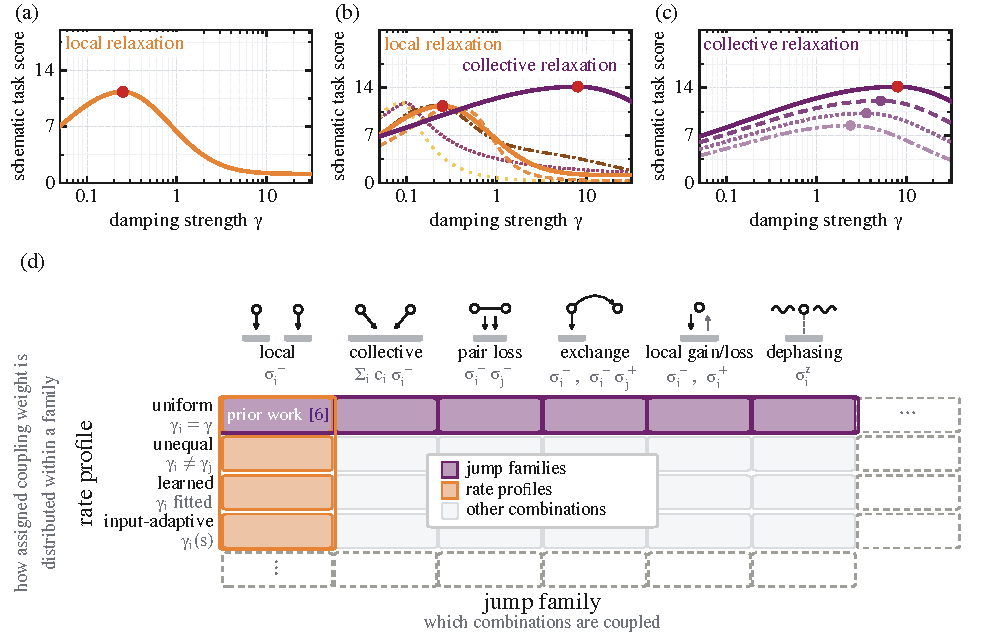
\includegraphics{figures/fig_designspace.pdf}};
% Figure-native PDF text cannot carry a manuscript-internal citation target
% through \includegraphics. This transparent, number-sized link sits exactly
% over the visible "6" in panel (d) and jumps to the Sannia et al. entry.
\begin{scope}[
  x={(designspacegraphic.south east)},
  y={(designspacegraphic.north west)}
]
\node[anchor=center,inner sep=0,outer sep=0] at (0.31685,0.34760)
  {\hyperlink{cite.Sannia2024}{\phantom{6}}};
\end{scope}
\end{tikzpicture}
\caption{\textbf{Dissipator geometry separates two complementary design
coordinates.}
\emph{(a)} Previous work primarily varies the overall strength of uniform
local relaxation~\cite{Sannia2024}. \emph{(b)} The jump family changes which
system combinations couple directly to the environment. \emph{(c)} The rate
profile redistributes coupling weight within a selected family.
\emph{(d)} Highlighted cells mark the two principal coordinate slices;
pale-gray cells show other combinations. Panels (a--c) show schematic task
scores, not fitted task data.}
\label{fig:space}
\end{figure*}

Figure~\ref{fig:space} maps these choices across the tested design space. The
local--collective example is intuitive, but the distinction must be defined at
the generator level.

Let \(\{F_\mu\}\) be a fixed set of traceless system operators with
\[
\Tr(F_\mu^\dagger F_\nu)=\delta_{\mu\nu}.
\]
Expanding every jump operator as
\[
L_k=\sum_\mu A_{k\mu}F_\mu,
\qquad
C=A^\dagger A\succeq0,
\]
makes this distinction invariant. The coefficient \(A_{k\mu}\) states how
strongly elementary action \(F_\mu\) contributes to environmental channel
\(k\). The matrix \(C\) records which elementary actions are coupled and how
the coupling weight is arranged among them. Equivalent remixings of the jump
list change the individual \(L_k\) and \(A\), but leave \(C\), and therefore
the dissipative generator, unchanged.
These coordinates are operational rather than globally orthogonal: a family
fixes the operator sector and allowed support of \(C\), whereas within-family
parameters set its nonzero weights and, where applicable, its direction within
that support. The construction is invariant under equivalent jump-list
remixings but remains relative to the declared elementary-operator basis.

For the one-body lowering block, the local--collective distinction takes the
form
\[
C_{\mathrm{lower}}^{\mathrm{local}}\propto I_N,
\qquad
C_{\mathrm{lower}}^{\mathrm{collective}}
  \propto \boldsymbol c\boldsymbol c^\dagger,
\]
where
\(\boldsymbol c=(c_1,\ldots,c_N)^{\mathsf T}\) parameterizes the shared
operator
\[
L_{\mathrm c}\propto\sum_i c_i\sigma_i^-.
\]
With nonzero local rates, \(I_N\) spans \(N\) independently coupled lowering
directions, whereas
\(\boldsymbol c\boldsymbol c^\dagger\) spans one directly coupled collective
direction. Rotating the written local jump operators cannot turn this
full-rank block into the rank-one shared block. Thus local and collective
relaxation are distinct generators.
\Needspace{3\baselineskip}
Unequal local relaxation instead changes the diagonal weights within the local
block and thus moves along the rate-profile axis.

\Needspace{4\baselineskip}
Table~\ref{tab:designs} is the exact catalogue of the tested environmental
actions; Fig.~\ref{fig:space} provides their intuitive map. We say gain/loss
rather than thermalization because its fixed transitions need not produce a
thermal state.

\subsection{Common structural normalization and paired comparison}

Unlike families contain different numbers and types of jump operators.
Assigning the same coefficient to every operator would therefore give more
total weight to a family merely because it contains more operators. We instead
fix
\begin{equation}
\mathcal B=\sum_k\Tr(L_k^\dagger L_k).
\label{eq:budget-intro}
\end{equation}
Each term is the squared operator size assigned to one environmental channel.
In the orthonormal basis above, \(\mathcal B=\Tr C\). Fixing
\(\mathcal B\) therefore provides a common structural bookkeeping scale: the
total assigned operator weight remains fixed while its organization changes.

For the principal fixed-\(\mathcal B\), common-protocol comparison, we vary
only the jump family. The Hamiltonian instance, input sequence, Pauli
observables, linear readout, training, selection, and test splits, and assigned
operator weight \(\mathcal B\) remain fixed.

This isolates structural change, not physical equivalence. In the one-body
local--collective comparison, fixed \(\mathcal B=\Tr C\) holds assigned coupling
weight fixed while changing the cross-site dissipative correlations encoded in
\(C\); it does not equalize activity,
the relaxation spectrum, energy flow, entropy production, implementation, or
hardware cost. The fixed-\(\mathcal B\) protocol therefore defines the cross-family
structural slice, while activity, gap, and operating-point controls additionally
validate only the local--collective memory ordering.

\subsection{Readout and computational tasks}

After each input interval, local Pauli expectations and same-axis two-qubit
correlations summarize the reservoir state,
\[
\{\langle X_i\rangle,\langle Y_i\rangle,\langle Z_i\rangle,
\langle X_iX_j\rangle,\langle Y_iY_j\rangle,\langle Z_iZ_j\rangle\}.
\]
They provide \(3N+3\binom{N}{2}\) features, or \(45\) at \(N=5\). Fixed-profile
structural experiments fit only the linear readout; separately identified profile and
operating-point studies also select dissipative parameters on data disjoint
from final testing. Appendix~\ref{app:experiment1} gives the ridge control.

Four benchmarks ask what information those features retain. Short-term memory
(STM)~\cite{JaegerSTM2001} reconstructs earlier inputs. NARMA-10
is the nonlinear autoregressive moving-average task of order ten. It tests a
nonlinear function of recent input history~\cite{AtiyaParlos2000}.
Parity combines binary memory with nonlinear processing. Mackey--Glass
forecasting~\cite{MackeyGlass1977} continues a chaotic signal in closed loop.
Capacity is maximized for STM and parity. Error is minimized for NARMA-10 and
forecasting.

For the adaptive-profile, finite-sampling, and alternative-control studies,
any additional mean matching, estimator choice, calibration, or selection
rule is stated explicitly.

\begin{table}[H]
\centering
\caption{\textbf{Dissipative designs.} The first two rows differ only in rate
profile. The displayed jump operators are convenient representatives of the
corresponding GKLS generators. Equivalent jump decompositions are not counted
as different designs.}
\label{tab:designs}
\footnotesize
\setlength{\tabcolsep}{3pt}
\renewcommand{\arraystretch}{1.06}
\begin{tabular}{@{}p{0.29\columnwidth}p{0.65\columnwidth}@{}}
\toprule
{\raggedright design\par}
& {\raggedright operators and direct environmental action\par}\tabularnewline
\midrule
{\raggedright\textbf{uniform local relaxation}~\cite{Sannia2024}\par}
& {\raggedright \(L_i=\sqrt{\gamma}\,\sigma_i^-\),
\(i=1,\ldots,N\). The same rate for every qubit; independent sitewise
relaxation and the reference design.\par}\tabularnewline
{\raggedright\textbf{unequal local relaxation}\par}
& {\raggedright \(L_i=\sqrt{\gamma_i}\,\sigma_i^-\),
\(i=1,\ldots,N\), with the \(\gamma_i\) not all equal. Independent sitewise
relaxation with qubit-dependent timescales.\par}\tabularnewline
\midrule
{\raggedright\textbf{collective relaxation}\par}
& {\raggedright \(\{\sum_i c_i\sigma_i^-\}\). One shared relaxation
channel.\par}\tabularnewline
{\raggedright\textbf{pair loss}\par}
& {\raggedright \(\{\sigma_i^-\sigma_j^-\}_{i<j}\). Joint two-excitation
removal.\par}\tabularnewline
{\raggedright\textbf{exchange-assisted relaxation}\par}
& {\raggedright
\(\{\sigma_i^-\}\cup\{\sigma_i^-\sigma_j^+\}_{i\ne j}\). Local lowering
supplemented by incoherent excitation exchange.\par}\tabularnewline
{\raggedright\textbf{local gain/loss}\par}
& {\raggedright \(\{\sigma_i^-,\sigma_i^+\}\). Fixed downward and upward
transitions.\par}\tabularnewline
{\raggedright\textbf{dephasing}\par}
& {\raggedright \(\{\sigma_i^z\}\). Phase randomization without excitation
loss.\par}\tabularnewline
\bottomrule
\end{tabular}
\end{table}

\begin{figure*}[!t]
\centering
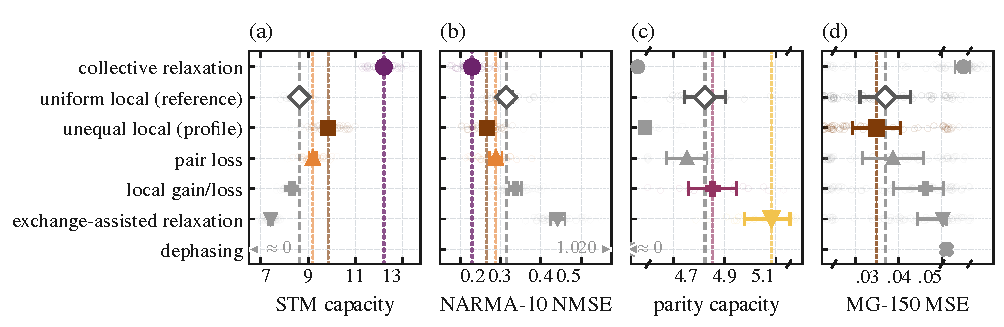
\includegraphics{figures/fig_task_scores.pdf}
\caption{\textbf{Different environmental couplings favor different
computations.}
Scores are shown for continuously driven \(N=5\) reservoirs. Each row
represents one dissipative design. Pale circles show individual reservoirs,
large symbols show the mean, and horizontal bars show pointwise \(95\%\)
intervals. The gray diamond and dashed line mark uniform local relaxation as
the reference. Colored symbols and matching dotted lines identify every design
whose mean outperforms that reference. Higher values are better for STM and
parity, whereas lower values are better for NARMA-10 and MG-150. The broken
axes in (c,d) enlarge the region where the designs differ while retaining all
observations. All designs are compared at the same assigned operator weight
\(\mathcal B\), which provides a common structural reference rather than
physical equivalence. Unequal local differs from the reference only through
its rate profile.}
\label{fig:map}
\end{figure*}

\section{\texorpdfstring{Computational consequences of coupling\\
organization}{Computational consequences of coupling organization}}
\label{sec:performance}

We traverse the two-coordinate design space of Fig.~\ref{fig:space}: first
across jump families, then across rate profiles within a family, and finally
across both axes jointly. We then ask whether exact-expectation differences
remain visible under finite measurement budgets.

\Needspace{6\baselineskip}
The fixed-weight task map establishes task-dependent computation before we
focus on its most strongly replicated consequence: the contrast in
readout-accessible recent-input memory between local and collective relaxation.

\subsection{Reference model and how to read the results}
\label{sec:results-guide}

Uniform local relaxation is the reference, with one equal-rate lowering
channel per qubit. Its family also includes unequal, learned, and
input-adaptive profiles. The main comparison uses the equal-phase rank-one
collective channel with \(c_i=1\) (Appendix~\ref{app:shared}). Profile-optimized
models instead learn within-family coefficients.

The four tasks retain their native metrics: STM and parity capacities are
maximized, whereas NARMA-10 NMSE and MG-150 MSE are minimized.

Figure~\ref{fig:map} reports the absolute \(N=5\) scores in each task's native
metric and favorable direction. The dashed vertical line in each panel marks
the uniform-local mean. Family-colored dotted lines and saturated markers
identify all designs with a better mean in that direction. Faint rings show
individual reservoir instances. The
panels retain their own scales and must be read independently.
Appendix Table~\ref{tab:map} gives the exact means and standard errors.

\subsection{Axis I: Jump-family choice changes the task profile}
\label{sec:map}

We first ask whether changing which system combinations couple to the
environment alters what the reservoir can compute.
\Needspace{5\baselineskip}
Each paired comparison
shares its Hamiltonian, input sequence, operating point, observables, readout,
data split, and structural budget \(\mathcal B\). Only the jump family
changes. Uniform local relaxation supplies the reference, while the
reset-encoded architecture introduced by Fujii and Nakajima (FN)~\cite{Fujii2017} is shown
separately as an external reservoir baseline.

The resulting task profiles differ, and no continuously driven design
dominates all four tasks. Collective relaxation leads STM and NARMA-10 under
the common protocol, but performs worse on parity and long closed-loop
forecasting. Exchange-assisted relaxation provides the clearest parity
improvement.

Under fixed \(\mathcal B\), the map shows protocol-specific specialization, not
a universal winner. A descriptive STM strength sensitivity preserves the
collective lead on the tested grid (Appendix~\ref{app:strength-sensitivity}).
We focus on local versus collective relaxation because it gives the cleanest
comparison within one lowering action and the strongest recurring memory change.

\subsection{Main jump-family case study: collective relaxation versus the
reference model}
\label{sec:collective-case}

We compare complete fixed-budget endpoints with
\(C_{\mathrm{lower}}^{\mathrm{local}}\propto I_N\) and
\(C_{\mathrm{lower}}^{\mathrm{collective}}\propto\boldsymbol c\boldsymbol
c^\dagger\). This endpoint comparison does not identify rank, delocalization,
coefficient-phase pattern, or drive alignment as separately causal.

\begin{figure*}[!t]
\centering
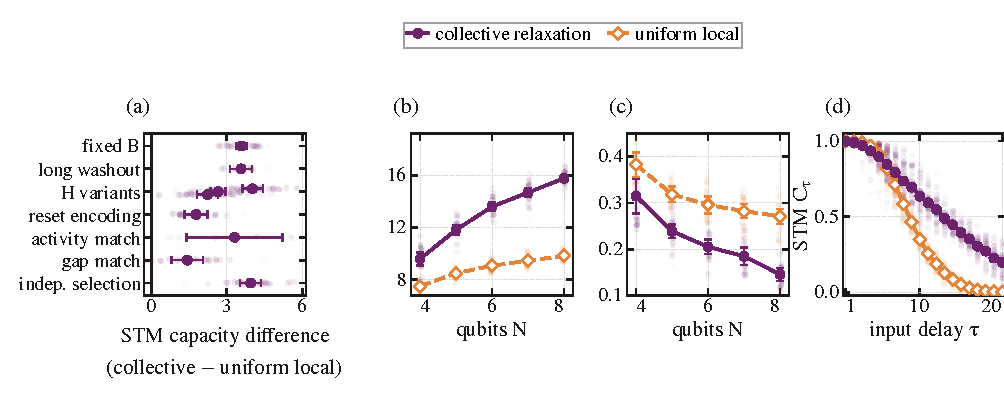
\includegraphics{figures/fig_collective_case.pdf}
\caption{\textbf{Collective relaxation preserves more usable input memory
than uniform local relaxation.}
\emph{(a)} STM gains under the main protocol and targeted controls. Values
above zero favor collective relaxation. \emph{(b,c)} STM capacity and
NARMA-10 error across the tested reservoir sizes. Collective relaxation
retains more memory and gives lower error. \emph{(d)} Memory from each previous
input. The slower purple decline shows that older inputs remain accessible for
longer. Pale marks show individual reservoirs. Large symbols and bars show
means and \(95\%\) intervals.}
\label{fig:collective-case}
\end{figure*}

At \(N=5\), collective relaxation increases STM from \(8.634\) to \(12.206\).
This is an absolute paired gain of \(3.57\) STM-capacity units and a relative
increase of \(41\%\), with a \(95\%\) interval of \([3.36,3.78]\) and \(32/32\)
paired wins. NARMA-10 NMSE decreases from \(0.315\) to \(0.229\), corresponding
to a \(27\%\) reduction in error, and improves in every paired reservoir.

\Needspace{7\baselineskip}
Figure~\ref{fig:collective-case}(b,c) provides a finite-size recurrence check of
the principal \(N=5\) ordering, not an asymptotic scaling analysis. Across 24
paired lineages per size, collective relaxation has the highest mean STM and
the lowest NARMA-10 error from \(N=4\) through \(N=8\).

Before interpreting the larger STM score as useful input memory, we test what
is being remembered. Removing every jump operator while retaining the
Hamiltonian, input protocol, and readout leaves STM and parity near zero,
raises NARMA-10 NMSE above one, and preserves initialization dependence
(Appendix Table~\ref{tab:map}). Coherent driving alone therefore reproduces
neither the task profile nor controlled forgetting. This unmatched diagnostic contrasts
with reset FN, which supplies non-unitary forgetting.

We next distinguish input memory from persistence of the starting state. The
same switched input sequence is applied from four widely separated states, and
their maximum trace distance is tracked. The convergence records in
Appendix~\ref{app:experiment1} show that local relaxation and pair loss
converge across \(N=4,5,6\) and
remain converged through the 1200-input continuation.

\Needspace{3\baselineskip}
Collective relaxation
converges more slowly, but reaches the same regime at the principal \(N=5\)
setting and in the tested \(N=6\) lineages.

\Needspace{4\baselineskip}
At \(N=5\), it approaches numerical
precision by the strict 800-input washout and reaches numerical precision
during the specified continuation to 1200 inputs.

\Needspace{9\baselineskip}
A ten-pair subset of the principal \(N=5\) lineages then uses the 800-input
washout before STM scoring. Cross-initialization differences are negligible,
while collective relaxation retains \(+3.564\,[3.124,4.004]\) STM units with
\(10/10\) wins (Fig.~\ref{fig:collective-case}(a)). For continuous-drive
NARMA-10, all 32 principal pairs are replayed after an independent 600-input
prefix, leaving the scored training and test rows unchanged. At the resulting
800-input washout, NMSE is \(0.315\) locally and \(0.230\) collectively, a
favorable paired difference of \(0.0851\,[0.0716,0.0986]\) with \(32/32\)
wins. The W800-minus-W200 effect change is
\(-0.00007\,[-0.00057,0.00043]\). Across four initial states on the first eight
pairs, the largest W800 NARMA-10 score spread is \(2.18\times10^{-5}\), far
below the smallest paired ground-state improvement, \(0.0148\). The stable
W800 endpoints therefore show that neither ordering is produced by the
residual initial-state dependence exposed at W200.

The comparison is also repeated under four spin-Hamiltonian ensembles that
change the interaction axis, drive axis, interaction form, or connectivity.
Every ensemble retains a positive collective-minus-reference STM difference,
ranging from \(+2.22\) to \(+4.02\) units
(Fig.~\ref{fig:collective-case}(a)). These replications preserve the continuous
encoding and Pauli readout, so they establish recurrence within the tested
driven-spin architecture. Appendix~\ref{app:experiment1} describes the
Hamiltonian variants and ridge control.

To test whether the ordering is tied to continuous-drive encoding, we replace
it with input-by-reset while retaining the \(N=5\) \(XX+Z\) processor, Pauli
readout, task definitions, and fixed structural budget. After an 800-input
washout, collective relaxation increases STM from \(4.596\) to \(6.369\), a
gain of \(1.773\,[1.312,2.235]\), and decreases NARMA-10 NMSE from \(0.673\)
to \(0.491\), a favorable reduction of \(0.182\,[0.144,0.220]\), with \(16/16\)
favorable pairs for both endpoints
(Fig.~\ref{fig:reset-architecture} and
Appendix~\ref{app:reset-architecture}). The ordering between local and
collective relaxation therefore recurs across two tested input architectures rather than being an
artifact of continuous driving.

\subsection{Axis II and joint design: rate profiles refine the chosen
jump family}
\label{sec:profiles}

Choosing a jump family does not fully specify the environmental coupling. A
second choice remains: how should the assigned coupling weight be distributed
within that family? We first keep the local-relaxation family
fixed and compare uniform, random unequal, learned static, and input-adaptive
rate profiles. All sites relax in every candidate, but they need not do so
equally. The profile-only unequal-local row in Appendix
Table~\ref{tab:map} reports the common-protocol comparison. The dedicated STM
sweep below uses the separately
specified profile-optimization protocol.

The uniform profile assigns the same rate to every site. A random unequal
profile introduces a fixed distribution of local timescales. A learned static
profile is fitted separately to each reservoir using validation data. An
adaptive profile varies with the current input. The static profiles share the
same mean rate. The adaptive profile is mean-matched over a fixed input grid
but may vary with the input.

\Needspace{8\baselineskip}
Figure~\ref{fig:profiles}(a) shows that rate redistribution changes STM without
changing the local-relaxation family. Random unequal rates improve on the
uniform-local reference, and reservoir-specific learning improves further.
The learned-minus-uniform gain is \(1.34\) units, with an interval of
\([1.13,1.55]\) and \(32/32\) wins. The adaptive profile gives only a marginal
additional gain under the matched restart and evaluation limits. This ordering
does not establish a general superiority of static profiles because the static
and adaptive parameterizations differ in dimension and stopping behavior.

Within-family tuning redistributes the diagonal rates in the local family,
whereas in the collective family it changes the coefficient vector
\(\boldsymbol c\) and thereby rotates the supported rank-one Kossakowski
direction. Both are well-defined, reproducible tuning operations.

The jump-family and rate-profile axes are not competing alternatives. We therefore
cross them directly by comparing uniform and learned profiles within both
local and collective relaxation at the same \(\mathcal B\).
Figure~\ref{fig:profiles}(b) displays this \(2\times2\) comparison. The vertical
separation shows the jump-family effect, the uniform-to-learned slope shows the
profile effect, and the different slopes show that the profile benefit depends
on the selected family.

\begin{figure}[H]
\centering
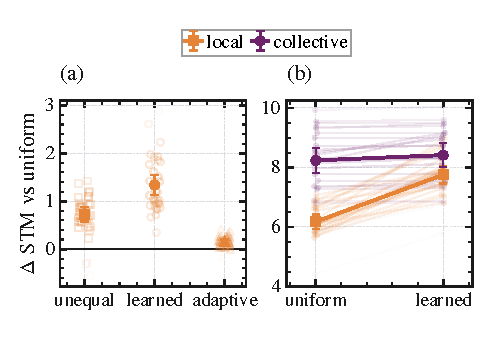
\includegraphics{figures/fig_profiles.pdf}
\caption{\textbf{Rate profiles tune memory within a chosen relaxation
family.}
\emph{(a)} Change in STM relative to uniform local rates for three alternative
profiles. Values above zero indicate improved memory. \emph{(b)} Learning the
rate profile increases STM for both local and collective relaxation, but the
increase is larger for local relaxation. Collective relaxation nevertheless
retains the higher STM overall. Lines connect the same reservoir before and
after learning. Pale marks show individual reservoirs. Large symbols and bars
show means and \(95\%\) intervals.}
\label{fig:profiles}
\end{figure}

The profile gain is larger for local relaxation. The difference between the
two gains is \(1.397\) STM units. All \(24/24\) paired values are positive, and
the familywise \(95\%\) interval is \([1.078,1.716]\). Collective relaxation
nevertheless remains higher after both profiles are learned. Profile
optimization refines the selected family by a family-dependent amount.
Appendix~\ref{app:experiment2} gives the parameterizations and inference scope.

\FloatBarrier
\subsection{Finite sampling determines experimental visibility}
\label{sec:measurement}

The preceding comparisons characterize the computation available to an exact
45-Pauli readout. An experiment observes finite measurement outcomes rather
than exact expectation values. We therefore ask a distinct question: at what
preparation budget do the differences created by coupling organization become
statistically visible?

\FiniteSamplePriorWork

At each step, independent sampling spends \(N_{\mathrm{prep}}=45q\) shots over
45 observables. Grouped sampling spends the same nominal budget in the global
\(X\), \(Y\), and \(Z\) bases and reuses each bitstring across 15 features.
Each design validates its ridge coefficient before one held-out evaluation.
``Preparations per step'' excludes replay of the preceding input history, so
Fig.~\ref{fig:sampling} studies measurement resolution, not end-to-end runtime.

At the exact-expectation endpoint, Fig.~\ref{fig:sampling} recovers the
collective-over-reference memory ordering from the jump-family comparison.
Grouped sampling resolves this contrast with one-sixteenth of the preparation
count needed by independent sampling. This gain is close to the 15-fold
feature reuse built into the estimator. It is a measurement advantage rather
than a hardware advantage specific to collective relaxation.

The finite-data curves also show why measurement design belongs in the
comparison. Sampling noise does not reduce every STM score by the same amount.
At the smallest independent-sampling budgets, pair loss appears best. Unequal
local relaxation leads at intermediate precision. Collective relaxation
emerges only after the observables are estimated accurately enough. Under
simultaneous inference across the complete comparison family, grouped sampling
resolves collective relaxation above every competitor only at the largest
finite budget. Independent sampling never resolves it as best on the tested
grid.

Appendix~\ref{app:experiment3} gives the estimator definitions, budget
parameterization, and simultaneous-inference scope.

\begin{figure}[!t]
\centering
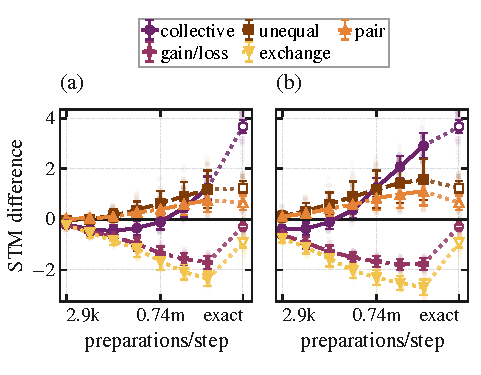
\includegraphics{figures/fig_sampling.pdf}
\caption{\textbf{Grouped measurements reveal memory differences with fewer
preparations.}
Each curve shows the STM difference from uniform local relaxation as the
measurement budget increases. Values above zero indicate more memory than the
reference, and values below zero indicate less. \emph{(a)} Observables are
measured independently. \emph{(b)} Compatible observables are measured
together, making the correct ordering visible with fewer preparations. Open
symbols show the exact results. Pale points show individual reservoir pairs.
Large symbols and bars show means and \(95\%\) intervals.}
\label{fig:sampling}
\end{figure}

Across these analyses, the memory advantage of collective over uniform local
relaxation is the strongest recurring jump-family effect.
Section~\ref{sec:interpretation} now examines which dynamics are consistent
with that contrast.

\section{\texorpdfstring{Dynamical interpretation of the\\
local and collective memory contrast}{Dynamical interpretation of the local
and collective memory contrast}}
\label{sec:interpretation}

Section~\ref{sec:performance} establishes the controlled computational ordering
independently of the interpretation below. Here we ask which dynamical picture
is consistent with it after the tested initial states have been forgotten, not
which microscopic ingredient is uniquely causal.

\subsection{Working physical picture}

The simplest distinction concerns how the reservoir reaches its environment.
Under uniform local relaxation, every spin has its own direct relaxation
channel. Under collective relaxation, the spins share one channel. The same
assigned coupling weight is therefore spread over several separate paths in
one case and concentrated into a common path in the other. Some combinations
of spin excitations then reach the collective channel only after the
Hamiltonian has mixed them with the directly coupled combination. They are not
permanently protected: coherent dynamics continue to move information between
these combinations. Appendix~\ref{app:shared} gives the corresponding
mathematical formulation and states its precise limits. The same interference
principle appears in collective emission and in network states that a shared
environment cannot address directly~\cite{Dicke1954,Cabot2018}.

This gives the working picture. A shared environmental channel directly
couples fewer combinations. Hamiltonian mixing provides indirect relaxation
routes for the others, so the resulting slower readout-visible responses can
preserve a longer accessible input history.

\subsection{Scalar controls for the memory contrast}

Fixing \(\mathcal B\) controls assigned operator weight, but it does not
equalize realized jump activity, the relaxation spectrum, or the operating
point preferred by each environmental-coupling design. We therefore ask whether any one of
these scalar differences is sufficient to explain the principal memory
contrast. These controls are not intended to factorize the generator into
uniquely causal structural ingredients. Figure~\ref{fig:collective-case}(a) summarizes the
fixed-\(\mathcal B\), activity-matched, gap-matched, and independently selected
comparisons. The STM contrast is positive in all four protocols.

The first control asks whether the shared channel wins simply because it
produces a different amount of realized jump activity. Local and collective
rates are calibrated separately to the same time-averaged expected activity
on an input stream without task labels, then frozen before task scoring. Every
calibration passes and the held-out activity difference is unresolved.
Collective relaxation still gains \(3.306\) STM units, with a \(95\%\)
interval of \([1.393,5.220]\) and \(8/8\) paired wins. Different mean jump
activity cannot by itself explain the memory contrast.
Appendix~\ref{app:activity-control} gives the calibration protocol.

The second control asks whether the shared channel remembers longer simply
because it relaxes more slowly. Before
any task stream is generated, each local rate is therefore calibrated to the
collective generator's Liouvillian gap at the constant input \(s=0.5\). This
gap is the slowest nonzero decay rate of that constant-input evolution and
provides one measure of relaxation speed. All 24 matches fall within the
prescribed tolerance.

Gap matching reduces the STM and NARMA-10 contrasts by \(62.1\%\) and
\(48.2\%\), respectively, showing that this timescale explains an important
part of the effect. It does not remove the ordering. Collective relaxation
retains \(1.424\) STM units with an interval of \([0.800,2.049]\) and \(20/24\)
wins, and the NARMA-10 difference remains resolved.
Figure~\ref{fig:scalar-controls}(b) in Appendix~\ref{app:experiment1}
resolves the same comparison by input delay. Matching the local rate restores
much of its memory tail, but
collective relaxation remains higher at long delays. The bands are pointwise
\(95\%\) intervals across the 24 paired reservoirs.
Appendix~\ref{app:gap-control} gives the calibration protocol.

Finally, a common setting could accidentally favor one jump family. Local and
collective relaxation therefore choose their own drive, input duration,
dissipative multiplier, and ridge coefficient, with disjoint data for
selection and final testing. Collective relaxation still leads by \(3.945\)
STM units, with an interval of \([3.523,4.368]\) and \(24/24\) wins. The
contrast does not require a shared operating point. The search is bounded
rather than global. Appendix~\ref{app:selection-control} gives the selection
protocol and bounded-search scope.

These controls rule out unequal mean activity, one representative decay rate,
and a common operating point as sole explanations of the principal ordering
between local and collective relaxation. They do not equalize the complete spectrum,
input-dependent propagator products, non-normal transients, energy flow,
entropy production, implementation effort, or hardware cost, and they were
not repeated for the full cross-family task map.

\subsection{Positive dynamical support}

\RelaxationTheoryPriorWork

Because STM is obtained by linear regression on the measured feature
trajectory, a dynamical component can contribute only if the input excites it
and it remains visible in the readout span. Fixed-input mode overlap tests
readout visibility. The switched-response kernel additionally includes input
excitation. The slower collective modes remain Pauli-visible, and after the
representative timescale is matched the switched response is concentrated into
fewer observable patterns.

Two additional checks connect this response to the coupling-organization
interpretation. Across six
process designs, slower midpoint relaxation usually accompanies more STM. A
separate sweep mixes local and collective loss continuously. Its selected
interior point improves on local relaxation in every fresh pair, demonstrating
robustness to residual local damping along this path. Together, the diagnostics
support one coherent account of the endpoint contrast.
Appendix~\ref{app:interpretation} reports their uncertainty.

\subsection{Scope of the explanation}

Along the fixed-weight interpolation, every interior one-body lowering block
retains Kossakowski rank \(N\) while STM changes, so rank alone is insufficient.
Learned profiles and the interpolation change several coordinates together.
Two matched rank-one interventions isolate Kossakowski orientation. The
primary \(N=5\) study finds more STM along the equal-phase end of a
prespecified path and against five zero-overlap controls. In a separately
generated \(N=6\) replication, rotating the equal-phase vector to the real,
sign-balanced direction \((1,1,1,-1,-1,-1)\), orthogonal to the uniform
site profile of the input drive, lowers STM by \(2.271\) units
\([1.826,2.717]\), with
\(24/24\) paired wins for equal phase and exact two-sided sign-test
\(p=1.19\times10^{-7}\). Kossakowski rank, nonzero spectrum and trace,
assigned operator weight, sitewise diagonal weights, coefficient magnitudes,
and every within-pair processor and data choice remain fixed
(Figure~\ref{fig:phase-direction} in Appendix~\ref{app:phase-direction}).
These invariants are
therefore insufficient to determine memory: Kossakowski orientation relative
to the fixed driven processor is an operative coupling-organization
coordinate. This
does not distinguish alignment with the input from alignment with the
coherent dynamics, or make equal phase or a response diagnostic universal.

Dephasing follows a different contraction mechanism. In the connected primary
model, it removes the measured signal after washout, which accounts for its
near-zero STM. Appendix~\ref{app:interpretation} gives the driven-dephasing
argument. It should not be folded into the shared-channel explanation.

\section{Discussion and conclusion}
\label{sec:discussion}

Previous dissipative QRC studies largely fix the environmental process and tune
only its strength. We show that this one-rate picture is incomplete. In the
finite spin reservoirs studied here, whether qubit transitions couple to
separate or shared channels, and how coupling is distributed among them,
changes which parts of the input history the measured output can recover. A
reservoir's connection to the environment is therefore part of its
computational design.

The clearest recurring comparison is between independent and shared
relaxation. With independent relaxation, each qubit couples to its own decay
channel. With shared relaxation, the environment couples directly to one
collective combination of transitions while the Hamiltonian can mix other
combinations into it. Shared relaxation makes more recent input history
recoverable and improves a nonlinear benchmark that depends on several earlier
inputs.

The cleanest intervention changes only the collective combination addressed by
an otherwise matched shared channel. Memory changes even though the channels
have the same number of coupled directions, the same nonzero coupling
strengths, the same total and per-qubit coupling weights, and identical
processors, inputs, and readouts. The same direction sensitivity appears at
both tested sizes. These comparisons identify what coarse summaries of
dissipation miss: the collective transition directly coupled to the
environment. Dynamical diagnostics and a gradual path between independent and
shared relaxation support this channel-selectivity picture, but do not
establish a unique microscopic mechanism.

The local-versus-shared ordering persists after longer washout, across the
tested sizes and Hamiltonians, with a different input encoding, and under
separate controls for average dissipative activity, a representative relaxation
rate, and operating-point selection. These checks make incomplete washout, one
processor or encoding, and the matched scalar differences insufficient
explanations. They establish a recurring contrast, not a universal advantage
over every environmental process.

Across memory, nonlinear processing, parity, and chaotic forecasting, different
dissipative designs favor different tasks. Redistributing a fixed coupling
budget within one design also changes memory. No process is best for every task.
Coupling organization is therefore a task-dependent design variable, not a
universal optimization rule.

Memory here means previous-input information that is linearly recoverable from
the specified Pauli measurements after washout, not an intrinsic quantum-memory
lifetime. The full task map concerns numerical five-qubit driven-spin
reservoirs. Recurrence from four to eight qubits does not establish asymptotic
scaling, and the four-qubit boundary is excluded from claims that the initial
state has been fully forgotten. Holding one common measure of coupling weight
fixed provides a controlled comparison, not dynamical, physical, or hardware
equivalence. The finite-measurement analysis includes projection noise and the
chosen estimators, but not drift, gate and readout errors, latency, or full
experimental cost. The analytical result on forgetting applies to driven
dephasing, not the shared-channel effect, and a generic common bath need not
realize the modeled collective process.

The result brings a familiar principle of dissipation engineering into temporal
quantum computation: designing the interaction between the system and the
environment~\cite{Poyatos1996,Verstraete2009,Pastawski2011,Harrington2022}. Shared
resonators, waveguides, and structured couplers suggest possible routes for
testing this coupling organization
~\cite{Cattaneo2019,Brehm2021,Sheremet2023,CattaneoPRX2023}. The next challenge
is to predict useful coupling patterns jointly from the Hamiltonian, input
encoding, environment, and measurement, then compare realizable couplers under
meaningful physical budgets in larger, noisy reservoirs. How coupling
organization interacts with non-Markovian memory is a separate open question.

Together, these results move dissipation in quantum reservoir computing from a
parameter to be tuned to a connection to be designed. The question is not only
how quickly information should decay, but which transitions should share a
route to the environment so that task-relevant history remains readable. For
temporal quantum processing, the way a reservoir forgets is part of how it
computes.


\acknowledgments{The authors gratefully acknowledge the research environment and
institutional support provided by the Quantum Applications and Research Laboratory
and the Mobile and Distributed Systems Group at Ludwig-Maximilians-Universit\"at
M\"unchen.}

\section*{Author contributions}
Markus Baumann conceived and led the study, developed the methodology and software,
performed the numerical experiments and formal analysis, curated the data, prepared
the visualizations, and wrote the original draft. Itamar Fink and Johannes Wittmann
contributed to the methodology, validation, interpretation of the results, and review
and editing of the manuscript. Claudia Linnhoff-Popien and Jonas Stein supervised the
project and contributed to its conceptual development. All authors approved the
final manuscript and its submission.

Anthropic's Claude Fable 5 and OpenAI's \mbox{GPT-5.6} were used as assistive tools for
checking selected intermediate derivations in the appendices, language editing, and
code debugging. All AI-assisted material was independently reviewed and verified by
the authors, who take full responsibility for the scientific content and final manuscript.

\Needspace{14\baselineskip}
\begingroup
\fontsize{9.5pt}{11.2pt}\selectfont
\bibliographystyle{quantum}
\bibliography{references}
\endgroup

\clearpage
\onecolumn
\appendix
\raggedbottom

\section{Reservoir model, dissipator construction, and shared methods}
\label{app:shared}
\label{sec:methods}

This appendix gives the shared definitions and numerical conventions, then
the additional controls and interpretation behind each analysis.

\subsection{Data and code availability}
\label{app:reproducibility}

All code, data, and analysis workflows for this work, together with the
manuscript source and figure inputs, are available at
\url{https://github.com/eybmits/qrc-dissipation-engineering}. The repository
documents the full protocol, including random seeds, Hamiltonian and input
definitions, data splits, parameter grids, solver and optimization settings,
and numerical tolerances. It also contains the calibration records,
convergence checks, and per-run outputs behind each reported number, so every
result in the paper can be inspected and reproduced.

\subsection{Collective process, pairing, and readout}
\label{app:collective-process}

The principal collective process uses one fixed vector in the main,
finite-size, Hamiltonian, activity-matched, and gap-matched comparisons:
\[
  c_i=1\quad(i=1,\ldots,N),\qquad
  \boldsymbol c=(1,\ldots,1),\qquad
  L_{\mathrm c}=\sqrt{\gamma}\sum_{i=1}^{N}\sigma_i^- .
\]
Thus the coefficients are real, have equal phase, and satisfy
\(\sum_i|c_i|^2=N\).  Only the separately identified profile-by-family check
fits a nonuniform collective profile.  The common target is the unit-rate
local value \(\mathcal B=N2^{N-1}\), giving \(\mathcal B=80\) at \(N=5\).
The finite-size study rematches this target separately at every \(N\).

The jump-family comparison uses independently drawn complete-graph couplings
\(J_{ij}\sim U[-1,1]\).  Unless a control explicitly changes an operating
point, \(h=\Delta t=0.5\), the reservoir starts in
\(\lvert0\cdots0\rangle\), and the STM and NARMA-10 sequences contain 200
washout, 600 training, and 400 test inputs. The task-specific parity and
MG-150 protocols are stated below. Comparisons are paired: for a given seed,
all dissipative designs see the same Hamiltonian, input sequence, targets,
and data split.  Variation across seeds therefore reflects both a new
reservoir and a new input sequence.

At \(N=5\), the readout contains the expectations of all one-qubit Pauli
operators and all same-axis two-qubit Pauli products.  These 45 measured
features, together with a bias, feed a linear classical readout.  The internal
quantum dynamics are not trained.  Continuous-input evolution is computed by
sparse matrix exponentiation.  The dense-grid approximation used only for
the bounded local-profile search is described in
Appendix~\ref{app:experiment2}.

\subsection{Tasks and what they probe}

Short-term memory (STM) asks whether a past input can be reconstructed from
the present reservoir state.  We sum the squared-correlation capacities for
delays \(1,\ldots,20\).  Larger values mean that more of the recent input
history remains linearly accessible.

NARMA-10 adds nonlinear temporal processing.  Its target obeys
\[
\begin{aligned}
y_k={}&0.3y_{k-1}+0.05y_{k-1}\sum_{j=1}^{10}y_{k-j}\\
&+1.5\tilde s_{k-10}\tilde s_{k-1}+0.1,
\qquad \tilde s=0.2s ,
\end{aligned}
\]
and is scored by normalized mean-squared error (NMSE), so smaller is better.
Parity uses binary input windows of length \(1,\ldots,7\) and 15 virtual
nodes per input interval.  It has separate 500/250/400
train/validation/test streams after 100 washout inputs.  Validation selects
the readout regularization before a train-plus-validation refit.

The forecasting target obeys the Mackey--Glass equation
\[
\dot x(t)=\frac{0.2x(t-17)}{1+x(t-17)^{10}}-0.1x(t).
\]
It is integrated by Euler steps of length one from the seeded delay history
\(x_t=1.2+0.01\xi_t\), with
\(\xi_t\overset{\mathrm{iid}}{\sim}\mathcal N(0,1)\). Every third Euler
iterate is retained, and the first 500 retained samples are discarded. After a
200-sample washout and 600-sample teacher-forced training prefix, the readout
is closed for 150 steps.  The affine scale
is fixed by the washout-plus-training prefix.  Only closed-loop predictions
fed back to the reservoir are clipped to \([0,1]\), while the held-out target
remains unclipped.

For Table~\ref{tab:map}, each continuously driven design and the external
reset-FN baseline uses 32 reservoirs for STM and NARMA-10, 16 for parity, and
64 for MG-150. The no-dissipation diagnostic uses 30, 30, 32, and 32
reservoirs, respectively.

\begin{table}[!t]
\centering
\caption{\textbf{Absolute scores for the fixed-\(\mathcal B\),
common-protocol comparison.}
Entries are mean \(\pm\) standard error. Arrows give the favorable direction,
and bold marks the best mean. Row groups distinguish external or diagnostic
comparisons, fixed-profile jump-family models, and a profile-only variation
within local relaxation. Task definitions and sample sizes are stated
immediately above.}
\label{tab:map}
\scriptsize
\setlength{\tabcolsep}{4pt}
\renewcommand{\arraystretch}{0.96}
\resizebox{\linewidth}{!}{%
\begin{tabular}{@{}lcccc@{}}
\toprule
model & STM \(\uparrow\) & NARMA-10 \(\downarrow\)
 & parity \(\uparrow\) & MG-150 \(\downarrow\)\\
\midrule
\multicolumn{5}{@{}l}{\emph{External and diagnostic comparisons}}\\
no dissipation
 & \(0.047\pm0.004\) & \(1.308\pm0.036\)
 & \(0.016\pm0.001\) & \(0.0697\pm0.0016\)\\
reset-encoded FN~\cite{Fujii2017}
 & \(10.106\pm0.260\) & \(0.367\pm0.012\)
 & \(2.295\pm0.125\) & \(0.115\pm0.008\)\\
\addlinespace[2pt]
\multicolumn{5}{@{}l}{\emph{Fixed-profile jump-family models}}\\
uniform local relaxation~\cite{Sannia2024}
 & \(8.634\pm0.069\) & \(0.315\pm0.008\)
 & \(4.822\pm0.038\) & \(0.0369\pm0.0029\)\\
collective relaxation
 & \(\mathbf{12.206\pm0.101}\) & \(\mathbf{0.229\pm0.006}\)
 & \(3.782\pm0.028\) & \(0.0969\pm0.0091\)\\
pair loss
 & \(9.203\pm0.082\) & \(0.289\pm0.007\)
 & \(4.752\pm0.037\) & \(0.0387\pm0.0035\)\\
local gain/loss
 & \(8.307\pm0.058\) & \(0.337\pm0.008\)
 & \(4.852\pm0.044\) & \(0.0462\pm0.0038\)\\
exchange-assisted relaxation
 & \(7.413\pm0.045\) & \(0.441\pm0.009\)
 & \(\mathbf{5.083\pm0.049}\) & \(0.0518\pm0.0038\)\\
dephasing
 & \(0.000\pm0.000\) & \(1.020\pm0.006\)
 & \(0.000\pm0.000\) & \(0.0599\pm0.0004\)\\
\addlinespace[2pt]
\multicolumn{5}{@{}l}{\emph{Profile-only variation within local relaxation}}\\
unequal local relaxation
 & \(9.845\pm0.119\) & \(0.266\pm0.007\)
 & \(4.366\pm0.071\) & \(\mathbf{0.0349\pm0.0028}\)\\
\bottomrule
\end{tabular}%
}
\end{table}

\subsection{Constructing and normalizing dissipative processes}

Table~\ref{tab:designs} gives the physical action of the six process families
and the unequal-rate variant.  Unequal local rates are drawn log-uniformly
from \([0.1,10]\) and rescaled to unit mean.  The collective coefficients are
the fixed equal-phase choice \(c_i=1\) stated in
Appendix~\ref{app:collective-process}.  Pair loss contains every \(i<j\).
Exchange-assisted relaxation combines local lowering with ordered,
excitation-conserving exchange jumps, assigning 40\% of \(\mathcal B\) to
the former and 60\% to the latter.  The local gain/loss process uses
downward/upward rates \(1/0.3\) before the common rescaling.  After
construction, one scalar rescales every completed design to the same
\(\mathcal B=\sum_k\Tr(L_k^\dagger L_k)\) as unit-rate uniform local
relaxation.

Section~\ref{sec:model} defines the fixed operator basis and Kossakowski matrix
used to compare generators independently of jump-list remixing. For the
one-body lowering families, write
\[
L_k=\sum_i A_{ki}\sigma_i^-,
\qquad
\Gamma=A^\dagger A\succeq0 .
\]
Then
\[
\mathcal B=2^{N-1}\Tr\Gamma .
\]
Thus fixed \(\mathcal B\) fixes \(\Tr\Gamma\). Uniform local relaxation has
rank \(N\), whereas the equal-phase collective channel has rank one. Kernel
directions are Kossakowski coupling directions, not decay modes of the full
Liouvillian; Hamiltonian mixing can provide indirect relaxation. The identity
above applies only to the one-body lowering block. Across unlike operator
sectors, fixed \(\mathcal B\) remains a structural control rather than an
equivalence of spectra, flows, or implementation cost.

\subsection{Statistical reporting}

All primary effects are computed as paired, instance-level differences and
oriented so that positive means improvement.  Unless stated otherwise, we
report the mean difference, a two-sided 95\% Student-\(t\) interval, and the
paired win count. For the non-reference cell comparisons, paired sign-flip
tests are corrected over the comparison family
with the Holm procedure~\cite{Holm1979}. Finite-size intervals use paired
bootstrap resampling. The profile and finite-sampling experiments use
simultaneous intervals because many related contrasts are examined together.

\FloatBarrier
\section{Jump-family computation and local--collective controls}
\label{app:experiment1}

The jump-family analysis asks whether changing the jump family changes
computation when the Hamiltonian, input, operating point, readout, and
\(\mathcal B\) are held fixed.  The broad map establishes the task dependence
of that jump-family choice.  The subsequent checks focus on the principal
collective-versus-local memory contrast.

\subsection{Fixed-\texorpdfstring{\(\mathcal B\)}{B} jump-family task map}

Figure~\ref{fig:map} and Table~\ref{tab:map} report the absolute
fixed-\(\mathcal B\) scores; Figure~\ref{fig:rank-map} gives the complementary
rank view.

A validation-selected readout control reuses the same STM and NARMA-10
trajectories but divides the 600 fitting rows into 450 training and 150
validation rows.  Each design and instance selects ordinary least squares or
a ridge value before refitting on all 600 rows.  The ordering is unchanged:
the collective design remains best on both tasks.  Thus the main ranking is
not an artifact of imposing one readout penalty on every process.

\begin{figure}[!t]
\centering
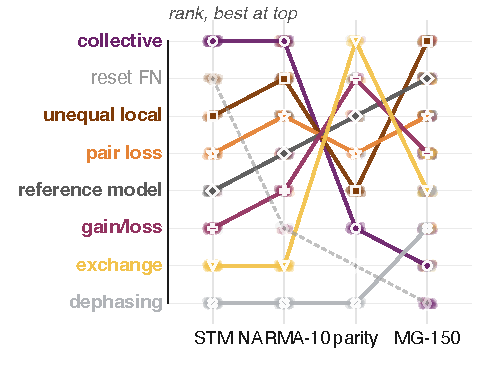
\includegraphics{figures/fig_map.pdf}
\caption{\textbf{Task-wise rankings confirm specialization rather than a
universal winner among the tested continuously driven designs.}
Ranks at \(N=5\) are induced by the absolute means in
Table~\ref{tab:map}; rank 1 is best within each task. Uniform local is the
reference. Colors follow the manuscript-wide dissipator palette; lines connect
identical designs only as visual guides. Dashed reset-based FN is an external,
unpaired baseline. Faint points rank the paired continuously driven seeds
against the fixed reset-FN mean; no seed points are assigned to that baseline.}
\label{fig:rank-map}
\end{figure}

\subsection{Robustness to the coherent dynamics}

The principal contrast was repeated in four paired \(N=5\) spin-Hamiltonian
ensembles: the primary \(XX+Z\) model with an \(X\) drive, a \(ZZ+X\) model
with a \(Z\) drive, an \(XY+Z\) model with an \(X\) drive, and an \(XX\) ring
with an \(X\) drive. The encoding and Pauli readout remain fixed.

\subsection{Replication under reset-based input encoding}
\label{app:reset-architecture}

To test whether the local--collective ordering depends on continuous-drive
encoding, we repeat the comparison in a reset-encoded reservoir. At input
step \(t\), qubit zero is replaced by
\[
 \rho_t^{+}
 = \lvert\psi(s_t)\rangle\!\langle\psi(s_t)\rvert_0
   \otimes \Tr_0(\rho_t),
 \qquad
 \lvert\psi(s)\rangle
 = \sqrt{1-s}\lvert0\rangle+\sqrt{s}\lvert1\rangle ,
\]
after which the autonomous \(XX+Z\) Hamiltonian evolves together with either
uniform local relaxation or the equal-phase collective channel. This changes
the input architecture: the reset is non-unitary and the input-dependent
transverse drive is absent during the evolution interval.

The strict comparison otherwise retains the principal \(N=5\) construction:
complete-graph couplings independently drawn from \(U[-1,1]\),
\(h=\Delta t=0.5\), \(\gamma=1\), \(\mathcal B=80\), i.i.d. inputs
\(s_t\sim U[0,1]\), the 45 Pauli features and bias, ridge \(10^{-8}\), STM
delays \(1,\ldots,20\), the same NARMA-10 target, and 600 training and 400
untouched test inputs. Within each of 16 fresh pairs, the local and collective
reservoirs share the Hamiltonian, input sequence, target, and data split. We
use an 800-input washout because
collective reset dynamics converge more slowly than their local counterpart.
Table~\ref{tab:reset-architecture} reports the strict task endpoints, and
Figure~\ref{fig:reset-architecture} shows their paired effects and
lag-resolved STM profile.

\begin{table}[H]
\centering
\caption{\textbf{Strict reset-encoded replication.} The effect is
collective-minus-local for STM and local-minus-collective for NARMA-10, so
positive values are favorable in both rows. Intervals are paired \(95\%\)
confidence intervals.}
\label{tab:reset-architecture}
\footnotesize
\setlength{\tabcolsep}{3.5pt}
\renewcommand{\arraystretch}{1.08}
\begin{tabular}{@{}lcccc@{}}
\toprule
task & local & collective & favorable effect & wins\\
\midrule
STM capacity
 & \(4.595912\) & \(6.369394\)
 & \(1.773\,[1.312,2.235]\) & \(16/16\)\\
NARMA-10 NMSE
 & \(0.672973\) & \(0.490933\)
 & \(0.182\,[0.144,0.220]\) & \(16/16\)\\
\bottomrule
\end{tabular}
\end{table}

\begin{figure}[H]
\centering
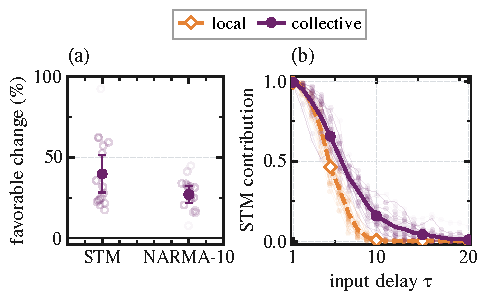
\includegraphics{figures/fig_reset_architecture.pdf}
\caption{\textbf{Replication under reset-based input encoding.}
\emph{(a)} Favorable paired relative change with respect to local relaxation
for STM capacity and NARMA-10 NMSE across 16 fresh paired reservoirs; positive
percentages denote larger STM or lower NMSE. Points show seeds, and filled
markers with bars show paired means and pointwise \(95\%\) \(t\) intervals.
\emph{(b)} Lag-resolved STM capacities after the strict 800-input washout;
faint lines and points are seeds, and thick lines and bands show means and
pointwise \(95\%\) \(t\) intervals. The fixed-budget comparison uses
\(\gamma=1\) and \(\mathcal B=80\).}
\label{fig:reset-architecture}
\end{figure}

Repeating both tasks and both dissipative models from the ground, fully
excited, maximally mixed, and Haar-random pure states gives a maximum score
range below \(7\times10^{-7}\); the largest trace distance at the 800-input
washout is \(1.3\times10^{-14}\), at numerical precision. The strict ordering
therefore reflects retained input history rather than the tested starting
state. It establishes that the effect transfers across the two tested input
architectures, not universal architecture independence. Nor does this
comparison imply that dissipation outperforms a reset-only unitary reservoir;
it isolates how two matched environmental-coupling designs shape usable memory.

\subsection{Finite size and loss of the initial state}

The finite-size study uses 24 fresh paired lineages at every
\(N=4,\ldots,8\).  Nested principal submatrices of an \(N=8\) coupling draw
are rescaled by \(\sqrt{4/(N-1)}\), and the Frobenius reference is rematched
within each size.  The number of measured Pauli features, excluding the fitted
bias, grows as
\[
F(N)=3N+3\binom{N}{2}.
\]
The sweep is intended as a finite-size robustness test of the paired
local--collective ordering, not as an analysis of asymptotic memory,
mixing-time, or Liouvillian scaling. STM is summed over a fixed 20-delay
horizon and therefore satisfies \(C_{\mathrm{STM}}\leq 20\) for every \(N\),
whereas \(F(N)\) grows with \(N\). Consequently,
\[
  \frac{C_{\mathrm{STM}}}{F(N)}
  \leq \frac{20}{3N+3\binom{N}{2}}.
\]
Even perfect recall at all tested delays would therefore have a decreasing
STM-per-feature ceiling. This ratio is not a neutral scaling or
resource-efficiency metric under the present protocol. The grouped readout
still requires only the three global \(X\), \(Y\), and \(Z\) settings, while
the fitted linear readout has \(F(N)+1\) inputs after including the bias.
Figure~\ref{fig:collective-case}(b) shows the absolute scores across size.

Because collective coupling can leave some combinations only indirectly
damped, we separately tested whether the reported memory could be residual
dependence on the starting state.  For each process and size, eight fresh
lineages at \(N=4,5,6\) were driven by identical switched input sequences from
the ground, fully excited, maximally mixed, and a Haar-random pure state.
Every checkpoint stores the largest trace and Pauli-feature distances over
the six initial-state pairs. Local and pair processes converge rapidly. A
continuation follows all 48 local and pair lineages at
\(N=4,5,6\) to 1200 inputs; their worst trace distance over steps 1100--1200
is \(6.85\times10^{-15}\).
\Needspace{4\baselineskip}
For collective relaxation at the principal \(N=5\)
setting, the worst trace distance falls from \(4.78\times10^{-4}\) after 200
inputs to \(1.32\times10^{-11}\) after 800. A separate continuation
follows all eight lineages to 1200 inputs and reaches
\(4.42\times10^{-15}\), below its declared \(10^{-14}\) gate. The slowly
forgetting collective \(N=4\) boundary case is excluded from
initialization-independent claims.

A stricter STM check uses ten principal-pair lineages, three distant initial
states, and washouts of 50, 200, and 800 inputs. A separate continuous-drive
NARMA-10 check uses all 32 principal pairs. For its W800 condition, a frozen
600-input prefix is placed before the unchanged canonical 1200-input sequence;
the final 200 washout inputs and the 600 training and 400 test rows are thus
identical to W200. Local and collective reservoirs share every input, target,
split, Hamiltonian, and readout choice within a pair. Ground-state scoring uses
all 32 pairs, and the first eight repeat both washouts from the ground, fully
excited, maximally mixed, and Haar-random states. The W200 scores must reproduce
the sealed principal values before the W800 aggregate is accepted. At W800,
local and collective NMSE are \(0.315\) and \(0.230\), respectively; the
local-minus-collective difference is \(0.0851\,[0.0716,0.0986]\), favorable in
all 32 pairs. Its change from W200 is
\(-0.00007\,[-0.00057,0.00043]\). The largest four-state collective score spread
at W800 is \(2.18\times10^{-5}\), below the smallest paired ground-state
improvement, \(0.0148\). The archive records every checkpoint and the
serialization-only amendment made before any non-audit score was generated.

\subsection{Matched expected jump activity}
\label{app:activity-control}

The fixed-\(\mathcal B\) comparison deliberately allows the realized jump
activity to differ.  To test whether this alone explains the memory result,
we calibrate the two processes using the time-averaged expectation
\[
\mathcal J=\frac{1}{T\Delta t}\sum_{t=1}^{T}\int_0^{\Delta t}
\sum_k\Tr\!\left[L_k^\dagger L_k\rho_t(\tau)\right]\,\mathrm d\tau .
\]
Local and collective rates are fitted separately to
\(\mathcal J_\star=0.5075\) on a shared, unlabeled input stream that is
independent of every task stream.  After 100 washout inputs, activity is
averaged over 150 intervals.  All 16 calibrations for eight fresh reservoir
pairs pass the predeclared 1.5\% tolerance before task scoring.

\subsection{Matched midpoint Liouvillian gap}
\label{app:gap-control}

A second control asks whether the result is only a consequence of the slowest
relaxation time at a representative constant input.  For each of 24 fresh
\(N=5\) Hamiltonians, the local rate is calibrated to the collective
Liouvillian gap at \(s=0.5\) before task inputs are generated.  All
calibrations satisfy the 0.5\% relative-error gate.

\subsection{Independent operating-point selection}
\label{app:selection-control}
\label{app:selection-ablation}

The third control lets local and collective relaxation select their own
operating points without using test data.  The bounded search varies the drive,
input duration, dissipative strength, and readout penalty over predeclared
grids.  A two-reservoir prescreen
advances eight settings per jump family.
Twelve disjoint reservoirs then select one setting and readout penalty per
process.  The final 24 reservoirs are opened only after these choices are
written.  The collective strength choice is additionally bracketed on the
selection set before the final test.

\begin{figure}[H]
\centering
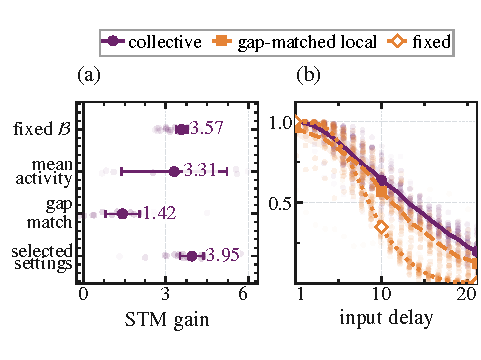
\includegraphics{figures/fig_scalar_controls.pdf}
\caption{\textbf{Targeted scalar controls preserve the local--collective
memory contrast.}
\emph{(a)} Collective-minus-reference STM effects for the fixed-\(\mathcal B\),
activity-matched, gap-matched, and independently selected protocols.
\emph{(b)} Lag-resolved STM at fixed \(\mathcal B\) and after matching the local
rate to the collective midpoint Liouvillian gap. Faint points show paired
seeds; bars and bands show the declared \(95\%\) intervals.}
\label{fig:scalar-controls}
\end{figure}

\subsection{Validation-selected scalar-strength sensitivity}
\label{app:strength-sensitivity}

The fixed-\(\mathcal B\) family map is a controlled jump-family slice rather
than a globally optimized ranking. In a complementary post hoc STM sensitivity
analysis, scalar strength is selected separately for six non-dephasing process
designs by leave-one-reservoir-out validation. All designs use the base
multiplier grid \(\{0.05,0.1,0.25,0.5,1,2,4\}\); uniform local and collective
relaxation also include \(8\) and \(16\), which bracket the collective optimum
at \(8\). The selected multipliers are \(8\) for collective, \(0.1\) for local
gain/loss and exchange-assisted relaxation, and \(0.25\) for uniform local,
unequal local, and pair loss; every curve is bracketed. Collective relaxation
has the largest mean across the 20 held-out scores, and 50,000 selection-aware
bootstrap draws give Bonferroni-simultaneous 95\% percentile intervals
whose lower endpoints are positive for its advantage over every competitor.
This supports the principal STM lead across the tested strength grid, but it
does not constitute a fully disjoint, task-wise optimized family ranking or a
four-task Pareto analysis.

\FloatBarrier
\section{Rate-profile optimization and comparison}
\label{app:experiment2}
\label{app:profiles}

The rate-profile analysis keeps the jump family fixed and changes only how
local relaxation strength is distributed across sites.  It therefore tests
the second coordinate of environmental-coupling organization independently of the jump-family
comparison.

\subsection{Within-family profile sweep}

The profile sweep uses \(N=5\), mean local rate 1.5,
\((h,\Delta t)=(0.5,0.5)\), and a shorter protocol tailored to profile
optimization.  It uses 100 washout inputs, 100 optimization-training inputs,
150 validation inputs, and 200 test inputs.  All static profiles have the
same arithmetic mean.  We compare a uniform reference with a random unequal
profile and a static profile learned on validation data.  A fourth model uses
the input-adaptive profile
\(\gamma_i(s)=\operatorname{softplus}(a_i s+b_i)\).  The adaptive profile is
matched only in mean over the frozen input grid, so its instantaneous
Frobenius strength may vary.

Static and adaptive profiles are optimized from seeded starts with fixed
evaluation limits and stopping rules.

\subsection{Does profile learning act the same way in every family?}

A separate \(2\times2\) check crosses local versus collective relaxation with
uniform versus learned profiles. Figure~\ref{fig:profiles}(b) displays the 24
paired trajectories and their mean changes.  Every candidate is normalized to
the same \(\mathcal B\), and exact continuous-input evolution replaces the dense
approximation.  For local relaxation, learning redistributes diagonal
sitewise rates.  For collective relaxation, it changes the coefficient vector
\(\boldsymbol c\) and thereby moves the supported one-dimensional
Kossakowski direction while preserving rank one.  The axes are therefore
operational and interacting design coordinates rather than a globally
orthogonal factorization. Inference uses simultaneous coverage over the eleven
declared contrasts.

\FloatBarrier
\section{Finite-sampling estimators and inference}
\label{app:experiment3}

The finite-sampling analysis asks whether the exact-expectation ordering remains
visible when Pauli features must be estimated from a finite number of
preparations.  It compares two estimators at the same nominal preparation
count, rather than treating shot noise as independent additive noise on every
feature.

\subsection{Two estimators at equal preparation count}

At \(N=5\), write \(N_{\mathrm{prep}}=45q\).  The independent estimator
spends \(q\) shots on each of the 45 observables.  The grouped estimator
instead spends \(15q\) shots in each global \(X\), \(Y\), and \(Z\) product
basis and reuses each measured bit string for all compatible one- and
two-qubit features.  Table~\ref{tab:sampling-estimators} emphasizes the
methodological difference without repeating the budget grid.

\begin{table}[H]
\centering
\caption{\textbf{Finite-sampling estimators at equal nominal preparation
count.} Grouping changes how measurement records are reused and therefore
preserves correlations between compatible Pauli estimates.}
\label{tab:sampling-estimators}
\footnotesize
\setlength{\tabcolsep}{6pt}
\renewcommand{\arraystretch}{1.12}
\begin{tabular}{@{}p{0.25\textwidth}p{0.33\textwidth}p{0.33\textwidth}@{}}
\toprule
 & independent observables & grouped Pauli settings\\
\midrule
recorded data
& one binomial estimate per feature
& full bit strings in \(X\), \(Y\), and \(Z\) bases\\
record reuse
& none across features
& one record informs all compatible features\\
covariance
& omitted by construction
& retained within each setting\\
modeled scope
& projection noise
& projection noise with grouping, without hardware noise\\
\bottomrule
\end{tabular}
\end{table}

\subsection{Training and simultaneous inference}

Six non-dephasing designs are evaluated on 20 paired reservoir and
measurement instances under both estimators.  Validation selects the readout
penalty from the predeclared grid before a
train-plus-validation refit.  We test \(q=64\times4^j\) for \(j=0,\ldots,6\),
so both estimators receive \(45q\) preparations per step.
Finite-budget intervals are simultaneous over every declared design-pair,
estimator, and budget contrast.  The exact-expectation endpoint is displayed
separately.

The curves in Figure~\ref{fig:sampling}(a,b) should therefore be read as a
resolution study. A design is distinguished from local relaxation only when
the simultaneous interval excludes zero, not merely when its mean is larger.
The model does not include acquisition latency, device drift, or gate and
readout errors.

\FloatBarrier
\section{Dynamical interpretation: support and limits}
\label{app:interpretation}

The following diagnostics test whether the observed response is consistent
with the shared-channel interpretation without claiming a unique microscopic
cause.

\subsection{Slow dynamics that remain visible to the readout}

For eight \(N=5\) local--collective lineages, the slowest right modes at five
constant inputs are projected onto the 45-Pauli readout span.  Collective
relaxation retains slower modes with larger overlap.  The paired differences
are \(0.338\,[0.239,0.436]\) in decay rate and
\(0.104\,[0.028,0.180]\) in readout-weighted retention. Because this omits
excitation weights and switched propagator products, it supports but does not
uniquely identify the shared-channel interpretation.

\subsection{Concentrated response under switched input}

Starting from synchronized trajectories, a complementary diagnostic applies
small input perturbations and follows the 45-feature response over 20 lags.
Collective relaxation concentrates this response in fewer observable
patterns than the matched local process.  Its effective rank is lower by
\(1.270\,[0.959,1.580]\), while the leading-pattern energy fraction is higher
by \(0.285\,[0.243,0.327]\).  The switched-input result supports the same
picture.  It is an empirical response kernel rather than a complete modal
decomposition.

\subsection{A gradual path from local to collective coupling}

To determine whether the endpoint contrast emerges along a continuous
coupling-organization path, we interpolate the dissipators at fixed Frobenius weight as
\(\D_\alpha=(1-\alpha)\D_{\mathrm{local}}
+\alpha\D_{\mathrm{collective}}\), with \(0\le\alpha\le1\).
Interior points are ranked on separate gap-only reservoirs before fresh task
streams are opened.  Increasing the collective component slows midpoint
relaxation and raises STM at \(N=4\) and \(5\).  The selected interior point
beats local relaxation in every fresh pair.  This links the endpoint result
to a continuous within-family deformation, not to a general selector for
unrelated processes.

\subsection{Why driven dephasing forgets uniformly}

The near-zero STM of the dephasing control admits a direct contraction
argument under the connectivity assumptions of the primary model.

\begin{proposition}[Uniform contraction of the driven dephasing model]
\label{prop:dephasing}
Let \(L_i=\sqrt{\gamma_i}Z_i\) with every \(\gamma_i>0\), let
\(\Phi_s=\exp(\Lind_s\Delta t)\) with \(\Delta t>0\), and suppose the nonzero
single-spin-flip matrix elements of \(H(s)\) connect the computational-basis
hypercube for every \(s\in[0,1]\). Then there is a \(\kappa<1\) such that
\[
\sup_{s\in[0,1]}
\left\|\Phi_s|_{\mathrm{Tr}=0}\right\|_{2\rightarrow2}\le\kappa .
\]
Here \(\|X\|_2=(\Tr X^\dagger X)^{1/2}\).  Hence
\(\|\rho_n-I/2^N\|_2\le\kappa^n\|\rho_0-I/2^N\|_2\) for any switched input
sequence and initial state.
\end{proposition}

\emph{Proof.}
For \(X_t=\exp(t\Lind_s)X\), the Hamiltonian commutator is skew-adjoint in the
Hilbert--Schmidt inner product, while the Hermitian-unitary jumps give
\(\frac{\mathrm d}{\mathrm dt}\|X_t\|_2^2
=-\sum_i\gamma_i\|[Z_i,X_t]\|_2^2\le0\).
Equality at \(\Delta t\) would make the norm constant, so every
\([Z_i,X_t]\) vanishes and \(X_t\) remains diagonal.  Its derivative can
remain diagonal only if \([H(s),X_t]=0\).  Hypercube connectivity then makes
\(X_t\) scalar.  Every nonzero traceless operator therefore contracts
strictly.  Attainment in finite dimension, continuity in \(s\), and
compactness of \([0,1]\) give one common \(\kappa<1\).\hfill\(\square\)

State differences are traceless, so the bound applies to every switched
sequence and all \(s\in[0,1]\).  It explains the dephasing zeros in
Table~\ref{tab:map} for the connected primary model, not arbitrary unital
dissipators.

\FloatBarrier
\section{Orientation within matched rank-one channels}
\label{app:phase-direction}

To vary the supported collective direction at fixed coarse channel invariants,
we use
\[
  c_i(f)=\exp\!\left[2\pi \mathrm{i}f(i-1)/5\right],\qquad
  f\in\{0,0.25,0.5,0.75,1\}.
\]
Here \(f=0\) is equal phase and \(f=1\) is orthogonal to the uniform direction.
Every condition has Kossakowski rank one, spectrum
\((5,0,0,0,0)\), unit diagonal, \(|c_i|=1\), magnitude IPR \(1/5\), and
\(\mathcal B=80\); four frozen phase-scrambled controls add zero-overlap
directions.

The confirmation uses 32 fresh paired reservoirs, excludes the pilot, and
shares Hamiltonian, input, target, split, and readout across all nine conditions
within each pair. After an 800-input washout, the unchanged protocol uses 600
training and 400 untouched test inputs, delays 1--20, 45 Pauli features, and
fixed ridge \(10^{-8}\). Four-state audits pass on the first eight lineages.

\begingroup
\setlength{\intextsep}{0pt}
\begin{figure}[H]
\centering
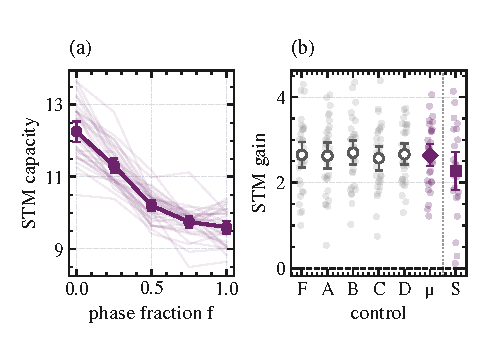
\includegraphics{figures/fig_phase_direction.pdf}
\caption{\textbf{Accessible memory depends on the matched rank-one direction.}
\emph{(a)} Prespecified \(N=5\) phase path. \emph{(b)} Equal-phase-minus-control
effects for five zero-overlap directions, their within-pair mean \(\mu\), and
the \(N=6\) sign-balanced replication S. Marks show pairs, means, and
\(95\%\) \(t\) intervals (32 and 24 pairs).}
\label{fig:phase-direction}
\end{figure}
\endgroup

Equal-phase STM is \(12.253\), versus \(9.604\) at the Fourier endpoint, a
paired difference of \(2.648\,[2.347,2.950]\) with \(32/32\) wins and
sign-flip \(p=1.0\times10^{-5}\). Against the within-pair mean of all five
zero-overlap directions, the gated effect is \(2.642\,[2.383,2.900]\), again
with \(32/32\) wins and \(p=1.0\times10^{-5}\). The ordered path and
validation-selected-ridge sensitivity agree.

\paragraph{Real sign-balanced replication at a second finite size.}
A separate 24-pair \(N=6\) endpoint replication compares
\(c_{+}=(1,1,1,1,1,1)\) with \(c_{\perp}=(1,1,1,-1,-1,-1)\), where
\(c_{+}^{\dagger}c_{\perp}=0\). At \(\mathcal B=192\), jump count, rank-one
spectrum \(\{6,0,0,0,0,0\}\), trace, diagonal weights, coefficient magnitudes,
processor, input, readout, data, and ridge rule remain fixed. All 24
ground/mixed-state audits and the first six four-state audits pass at W800.
Equal-phase STM is \(13.626\) versus \(11.354\), a paired gain of
\(2.271\,[1.826,2.717]\) with \(24/24\) wins and exact sign-test
\(p=1.19\times10^{-7}\); every delay-wise mean difference is positive. Thus
orientation affects accessible memory beyond these coarse matches, without
implying scaling, global optimality, or a unique mechanism.


\end{document}
